\begin{figure}[htbp]
  \centering
  \begin{adjustbox}{max width=\textwidth}
    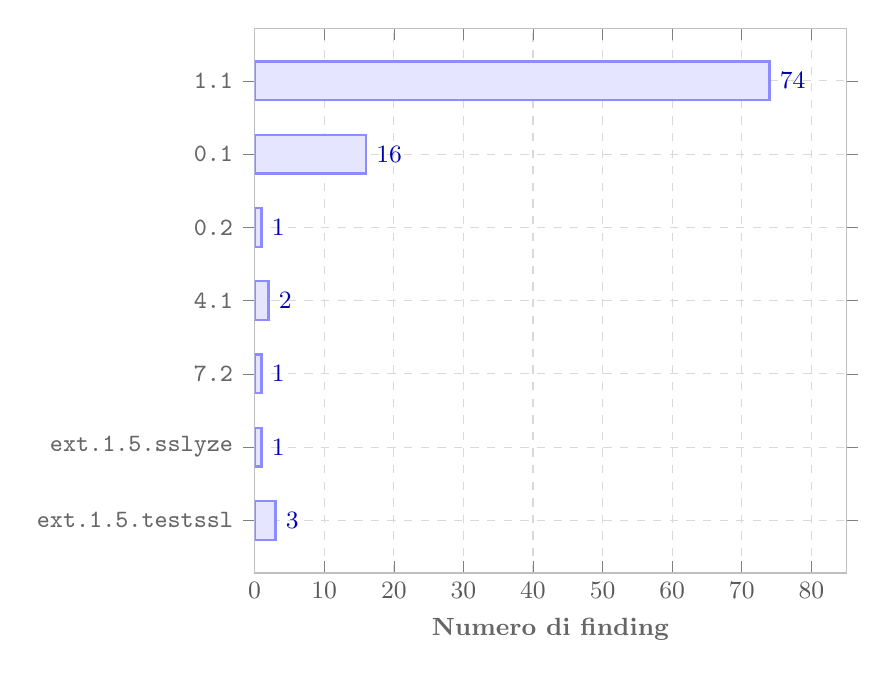
\begin{tikzpicture}
      \begin{axis}[
          xbar,
          width=0.75\textwidth, % <-- CORREZIONE: Lascia il 25% di spazio per le etichette laterali
          height=8.5cm,
          bar width=14pt,
          %
          % Setup Asse X
          xmin=0, xmax=85,
          xtick={0,10,20,30,40,50,60,70,80},
          xlabel={Numero di finding},
          xlabel style={font=\small\bfseries, text=gray!80!black},
          tick label style={font=\small, text=gray!70!black},
          %
          % Setup Asse Y
          symbolic y coords={{ext.1.5.testssl},{ext.1.5.sslyze},{7.2},{4.1},{0.2},{0.1},{1.1}},
          ytick=data,
          yticklabel style={font=\small\ttfamily, text=gray!80!black},
          enlarge y limits=0.12,
          %
          % Griglia
          grid=major,
          grid style={dashed, gray!30},
          axis line style={gray!50},
          %
          % Numeri a fianco delle barre
          nodes near coords,
          nodes near coords align={horizontal},
          every node near coord/.style={font=\small\bfseries, text=blue!70!black},
        ]

        \addplot[fill=blue!10, draw=blue!45, thick] coordinates {
            (3,{ext.1.5.testssl})
            (1,{ext.1.5.sslyze})
            (1,{7.2})
            (2,{4.1})
            (1,{0.2})
            (16,{0.1})
            (74,{1.1})
          };
      \end{axis}
    \end{tikzpicture}
  \end{adjustbox}
  \caption{Distribuzione dei 98 finding per test nell'assessment di validazione.}
  \label{fig:finding-distribution}
\end{figure}
